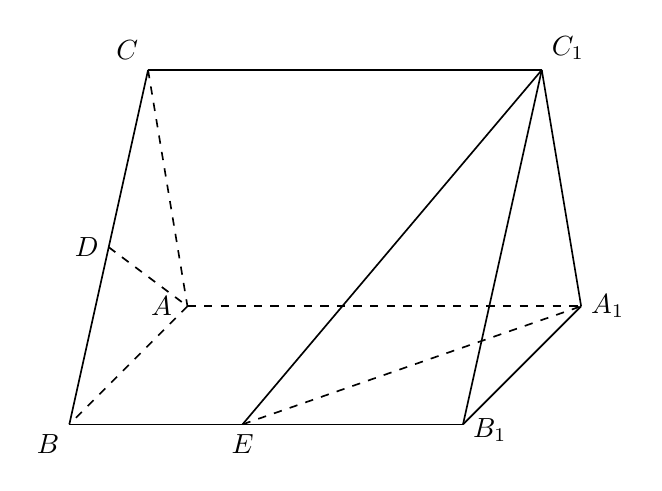
\begin{tikzpicture}[x=1cm,y=1cm,font=\normalsize,line width=.6pt]
\coordinate (A) at (1.5,1.5);
\coordinate (B) at (0,0);
\coordinate (C) at (1.0,4.5);
\coordinate (D) at (0.5,2.25);
\coordinate (E) at (2.2,0);
\coordinate (Bone) at (5.0,0);
\coordinate (Aone) at (6.5,1.5);
\coordinate (Cone) at (6,4.5);
% left triangular face ABC
\draw[solid] (B) -- (C);
\draw[dashed] (C) -- (A);
\draw[dashed] (A) -- (B);
\draw[dashed] (D) -- (A);
% lateral edges
\draw[solid] (C) -- (Cone);
\draw[dashed] (A) -- (Aone);
\draw[solid] (B) -- (Bone);
% right triangular face A1B1C1
\draw[solid] (Cone) -- (Aone);
\draw[solid] (Aone) -- (Bone);
\draw[solid] (Bone) -- (Cone);
% point E on BB1 and segments E-C1, E-A1
\draw[solid] (E) -- (Cone);
\draw[dashed] (E) -- (Aone);
\node[left,xshift=-2.00bp,yshift=0.00bp] at (A) {$A$};
\node[below left] at (B) {$B$};
\node[above left] at (C) {$C$};
\node[left] at (D) {$D$};
\node[below] at (E) {$E$};
\node[right,xshift=0.00bp,yshift=-2.00bp] at (Bone) {$B_{1}$};
\node[right] at (Aone) {$A_{1}$};
\node[above right] at (Cone) {$C_{1}$};
\end{tikzpicture}
